\documentclass{beamer}

\usepackage{lipsum}
\usepackage{multicol}
\usetheme{ucla}
\usepackage{graphicx}
\usepackage{listings}
\usepackage{verbatim}
\linespread{1.5}

\usepackage{amsmath, amsthm, amssymb, latexsym}

%\newtheorem{definition}{Definition}

\title{Lecture 1}
\author{Charles Rambo}
\institute{UCLA Anderson School of Management}
\date{2023}
\location{Los Angeles, California}

% Turn on slide numbers:
\showSlideNumber{}

\AtBeginSection[]
{
    \begin{frame}
        \frametitle{Table of Contents}
        \tableofcontents[currentsection]
    \end{frame}
}


\begin{document}

\insertTitleSlide


\begin{frame}
\frametitle{Table of Contents}
\tableofcontents
\end{frame}

\section{Python}

\begin{frame}
\frametitle{Python Installation}
\begin{itemize}
\item We'll be using Python.
\item If you haven't used Python before, I suggest downloading Anaconda at  \url{https://www.anaconda.com/download}
\end{itemize}
\begin{center}

\includegraphics[scale = 0.1]{anaconda.png}
\end{center}
\end{frame}

\begin{frame}
\frametitle{Anaconda}

After you've installed and opened Anaconda, a screen like this will appear. You have several choices for IDEs. Spyder is useful for data analysis. Jupyter Notebook is popular for explanatory work, so students and teachers tend to use it. You can use any IDE.
\begin{center}

\includegraphics[scale = 0.1]{anaconda2.png}
\end{center}
\end{frame}

\frame{
\frametitle{Packages}

{
%\linespread{1.5}
Several popular modules (packages) are preinstalled in Anaconda. 
\begin{itemize}
\item {\it NumPy}:  Useful math functions.
\item {\it Matplotlib:} Graphing. Somewhat quirky syntax but very popular nonetheless. 
\item {\it SciPy}: Scientific computing functions.
\end{itemize}
}
}

\frame{
\frametitle{Package Installation} 
To install a new package, go into Terminal, and type 
\begin{center}
{\tt pip install \ldots}
\end{center}
In this example, I'm upgrading pandas. Your Terminal will probably look different.
\begin{center}
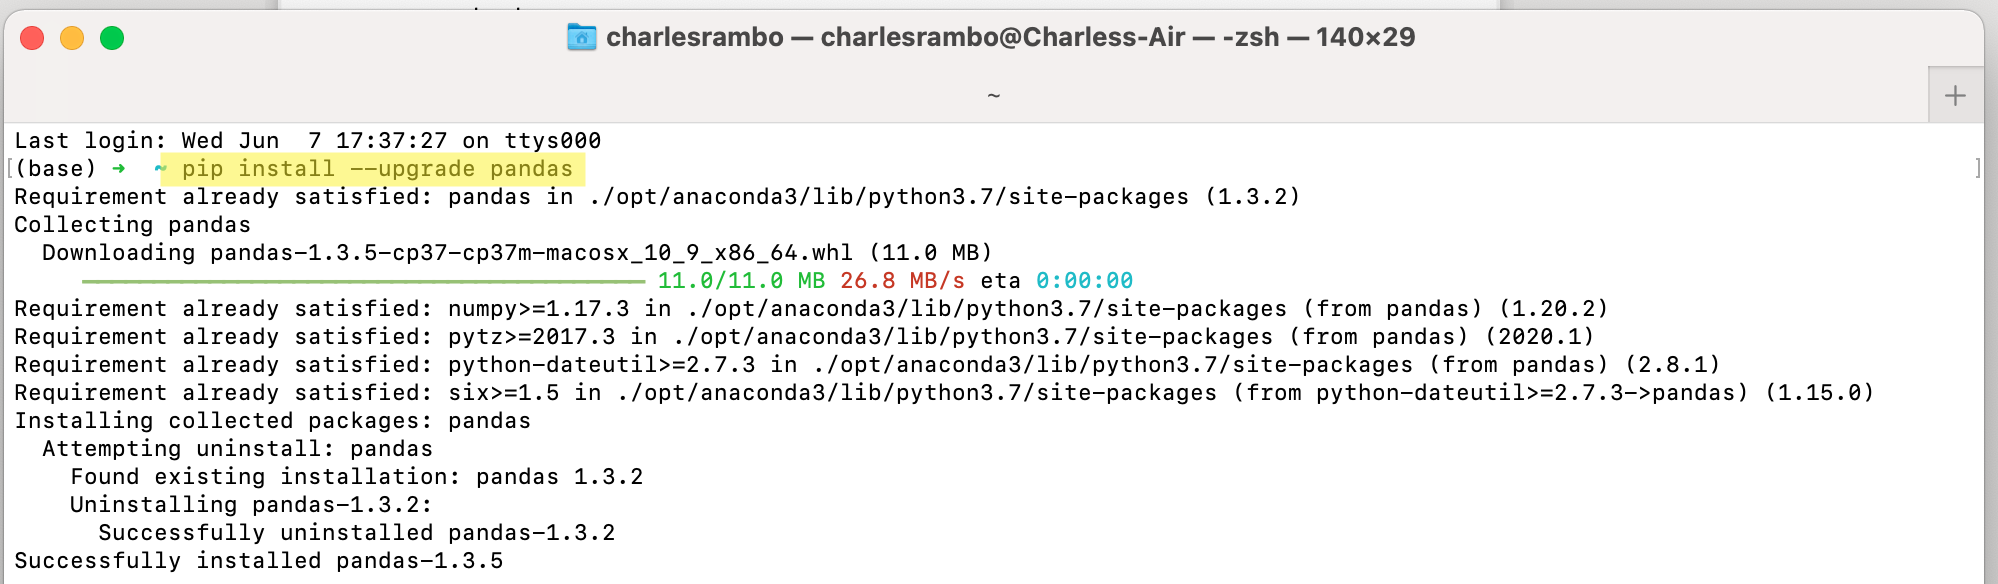
\includegraphics[scale = 0.2]{pip.png}
\end{center}
}


\begin{frame}[fragile]
\frametitle{Python Graphing Example}

\begin{example} 
Let $f(x) = x^2 + 1$. Use Python to graph $f$ on the domain $[-1, 2]$.
\end{example}

{
\linespread{0.8}
{\bf Solution.}  
{\tiny
\begin{verbatim*}
# Import modules 
import numpy as np
import matplotlib.pyplot as plt

# These steps add style; less important

# Use latex
plt.rcParams['text.usetex'] = True

# Use Seaborn style
plt.style.use('seaborn')

# Define f
def f(x):
    return x**2 + 1

# Another option is to use a lambda function
# f = lambda x: x**2 + 1

# Get 100 x-values on [-1, 2]
x_vals = np.linspace(-1, 2, 100)

# Use list comprehension to get y-values
y_vals = [f(x) for x in x_vals]

\end{verbatim*}
}}
\end{frame}

\begin{frame}[fragile]
\frametitle{Python Graphing Example Cont.}
{
\linespread{0.8}
\small

\begin{verbatim*}

# Generate the plot
plt.plot(x_vals, y_vals)

# Label the x-axis
plt.xlabel(r'$x$')

# Label the y-axis
plt.ylabel(r'$y$')

# Give the graph a title
plt.title(r'Graph of $y = x^2 + 1$')

# Save the figure
plt.savefig(r'[location on machine]')

# Display the plot
plt.show()
\end{verbatim*}
}

\end{frame}

\begin{frame}
\frametitle{Python Graphing Result}
\begin{center}
\includegraphics[scale = 0.5]{ex1.png}
\end{center}
\end{frame}

\begin{frame}[fragile]
\frametitle{Python Optimization Example}
\begin{example}
Use Python to find the minimum of $f(x) = x^2 + 1$ on the interval $[-1, 2]$.
\end{example}

{\bf Solution.} From the graph on the previous page, we know that the minimum is $y = 1$ which occurs when $x = 0$. But let's use Python to verify this. Suppose the code above is still in our local environment. 

\end{frame}

\begin{frame}[fragile]
\frametitle{Python Optimization Example Cont.}

{
\linespread{0.8}
\small
\begin{verbatim*}
# Import minimize from scipy
from scipy.optimize import minimize

# Minimize function; set bounds equal to the domain
minimize(f, x0 = [1], bounds = [(-1, 2)])
\end{verbatim*}
}
The output is shown below. 
{
\linespread{0.8}
\small
\begin{verbatim*}
fun: array([1.])
 hess_inv: <1x1 LbfgsInvHessProduct with dtype=float64>
      jac: array([0.])
  message: b'CONVERGENCE: NORM_OF_PROJECTED_GRADIENT_<=_PGTOL'
     nfev: 8
      nit: 2
   status: 0
  success: True
        x: array([-2.20890595e-10])
\end{verbatim*}
}
\end{frame}

\section{Limits}

\frame{
\frametitle{Definition}

\begin{Definition}
{
\linespread{1}
\begin{enumerate}
\item[(a)] Define $\displaystyle\lim_{x\to a} f(x) = L$ to mean for all $\epsilon > 0$ there exists a $\delta > 0$ such that
$$
0 < |x - a| < \delta\qquad\text{implies}\qquad \left|f(x) - L\right| <\epsilon.
$$
\item[(b)] Define $\displaystyle\lim_{x\to \infty} f(x) = L$ to mean for all $\epsilon > 0$ there exists an $N$ such that
$$
x \geq N \qquad\text{implies}\qquad \left|f(x) - L\right| <\epsilon.
$$
\item[(c)] Define $\displaystyle\lim_{x\to -\infty} f(x) = L$ to mean 
for all $\epsilon > 0$ there exists an $N$ such that
$$
x \leq N \qquad\text{implies}\qquad \left|f(x) - L\right| <\epsilon.
$$
\end{enumerate}
}
\end{Definition}
}


\begin{frame}[t]
\frametitle{Using the Definition}
\begin{Example}
Prove
$$
\displaystyle\lim_{x\to\infty} \frac{1}{x^p} = 0
$$
for all $p > 0$.
\end{Example}
\end{frame}

\frame{
\frametitle{Properties of Limits}
\begin{Theorem} 
Suppose $a$ is in the interval $[-\infty, \infty]$. Let
$$
\lim_{x\to a} f(x) = L_1,\qquad\text{and}\qquad\lim_{x\to a} g(x) = L_2.
$$
\begin{enumerate}
\item[(a)] $\displaystyle\lim_{x\to a} \alpha f(x) + \beta g(x) = \alpha L_1 + \beta L_2$ for any real constants $\alpha$ and $\beta$
\item[(b)] $\displaystyle\lim_{x\to a} f(x) \cdot g(x) = L_1\cdot L_2$
\item[(c)] $\displaystyle\lim_{x\to a} \frac{1}{f(x)} = \frac{1}{L_1}$ if $L_1 \neq 0$.
\end{enumerate}
\end{Theorem}
}

\begin{frame}
\frametitle{Useful Limits}
\begin{Theorem}
Suppose $p > 0$.
\begin{enumerate}
\item[(a)] $\displaystyle\lim_{x\to\infty} \frac{1}{x^p} = 0$
\item[(b)] $\displaystyle\lim_{x\to\infty} p^{1/x} = 1$
\item[(c)] $\displaystyle\lim_{x\to\infty} x^{1/x} = 1$
\item[(d)] If $ a > 0$, $\displaystyle\lim_{x\to 0} \frac{a^x - 1}{x} = \ln a$
\item[(e)] If $|r| < 1$, then $\displaystyle\lim_{x\to\infty} r^x = 0$
\end{enumerate}
\end{Theorem}
\end{frame}

\frame{
\frametitle{Python Example}
\begin{Example}
Define
$$
f(x) = \begin{cases} 
\sin\left(\frac{1}{x}\right),	&	x\neq 0\\ 0,	&	x = 0.
\end{cases}
$$
Graph $f$ in Python to see that $\displaystyle\lim_{x\to 0} f(x)$ does not exist.
\end{Example}
}

\begin{frame}[fragile]
\frametitle{Python Example Cont.}
{
\linespread{0.8}
\tiny
\begin{verbatim*}
# Import modules 
import numpy as np
import matplotlib.pyplot as plt

# Use latex
plt.rcParams['text.usetex'] = True

# Use Seaborn style
plt.style.use('seaborn')

# Define f
f = lambda x: 0 if x == 0 else np.sin(1/x)   
        
# Let's graph on the interval [-pi, pi]
x_vals = np.arange(-np.pi, np.pi, np.pi/192)

# Calculate the y-values
y_vals = [f(x) for x in x_vals]

# Generate the plot
plt.plot(x_vals, y_vals)

# Label the x-axis
plt.xlabel(r'$x$')

# Label the y-axis
plt.ylabel(r'$y$')

# Give the graph a title
plt.title(r'Graph of $y = f(x)$')

# Save the figure
plt.savefig(r'[location on machine]')

# Display the plot
plt.show()
\end{verbatim*}
}
\end{frame}

\begin{frame}
\frametitle{Python Example Result}
The graph isn't perfect, but it's enough to see that $f$ doesn't approach anything in particular as $x$ approaches 0.
\begin{center}
\includegraphics[scale = 0.4]{ex2.png}
\end{center}
\end{frame}


\section{Continuity} 

%\subsection{Basics}

\begin{frame}
\frametitle{Continuity}
\begin{Definition}
\begin{enumerate}
\item[(a)] A function $f$ is continuous at $a$ if $\displaystyle \lim_{x\to a} f(x) = f(a)$.
\item[(b)] A function $f$ is continuous on the set $A$ if
$$
a\in A\qquad\text{implies}\qquad \lim_{x\to a} f(x) = f(a).
$$
\end{enumerate}
\end{Definition}
\end{frame}

\begin{frame}
\frametitle{Continuity Idea}
Continuous functions have no breaks, i.e. if you were to draw them you would never need to lift your pencil. 
\begin{center}
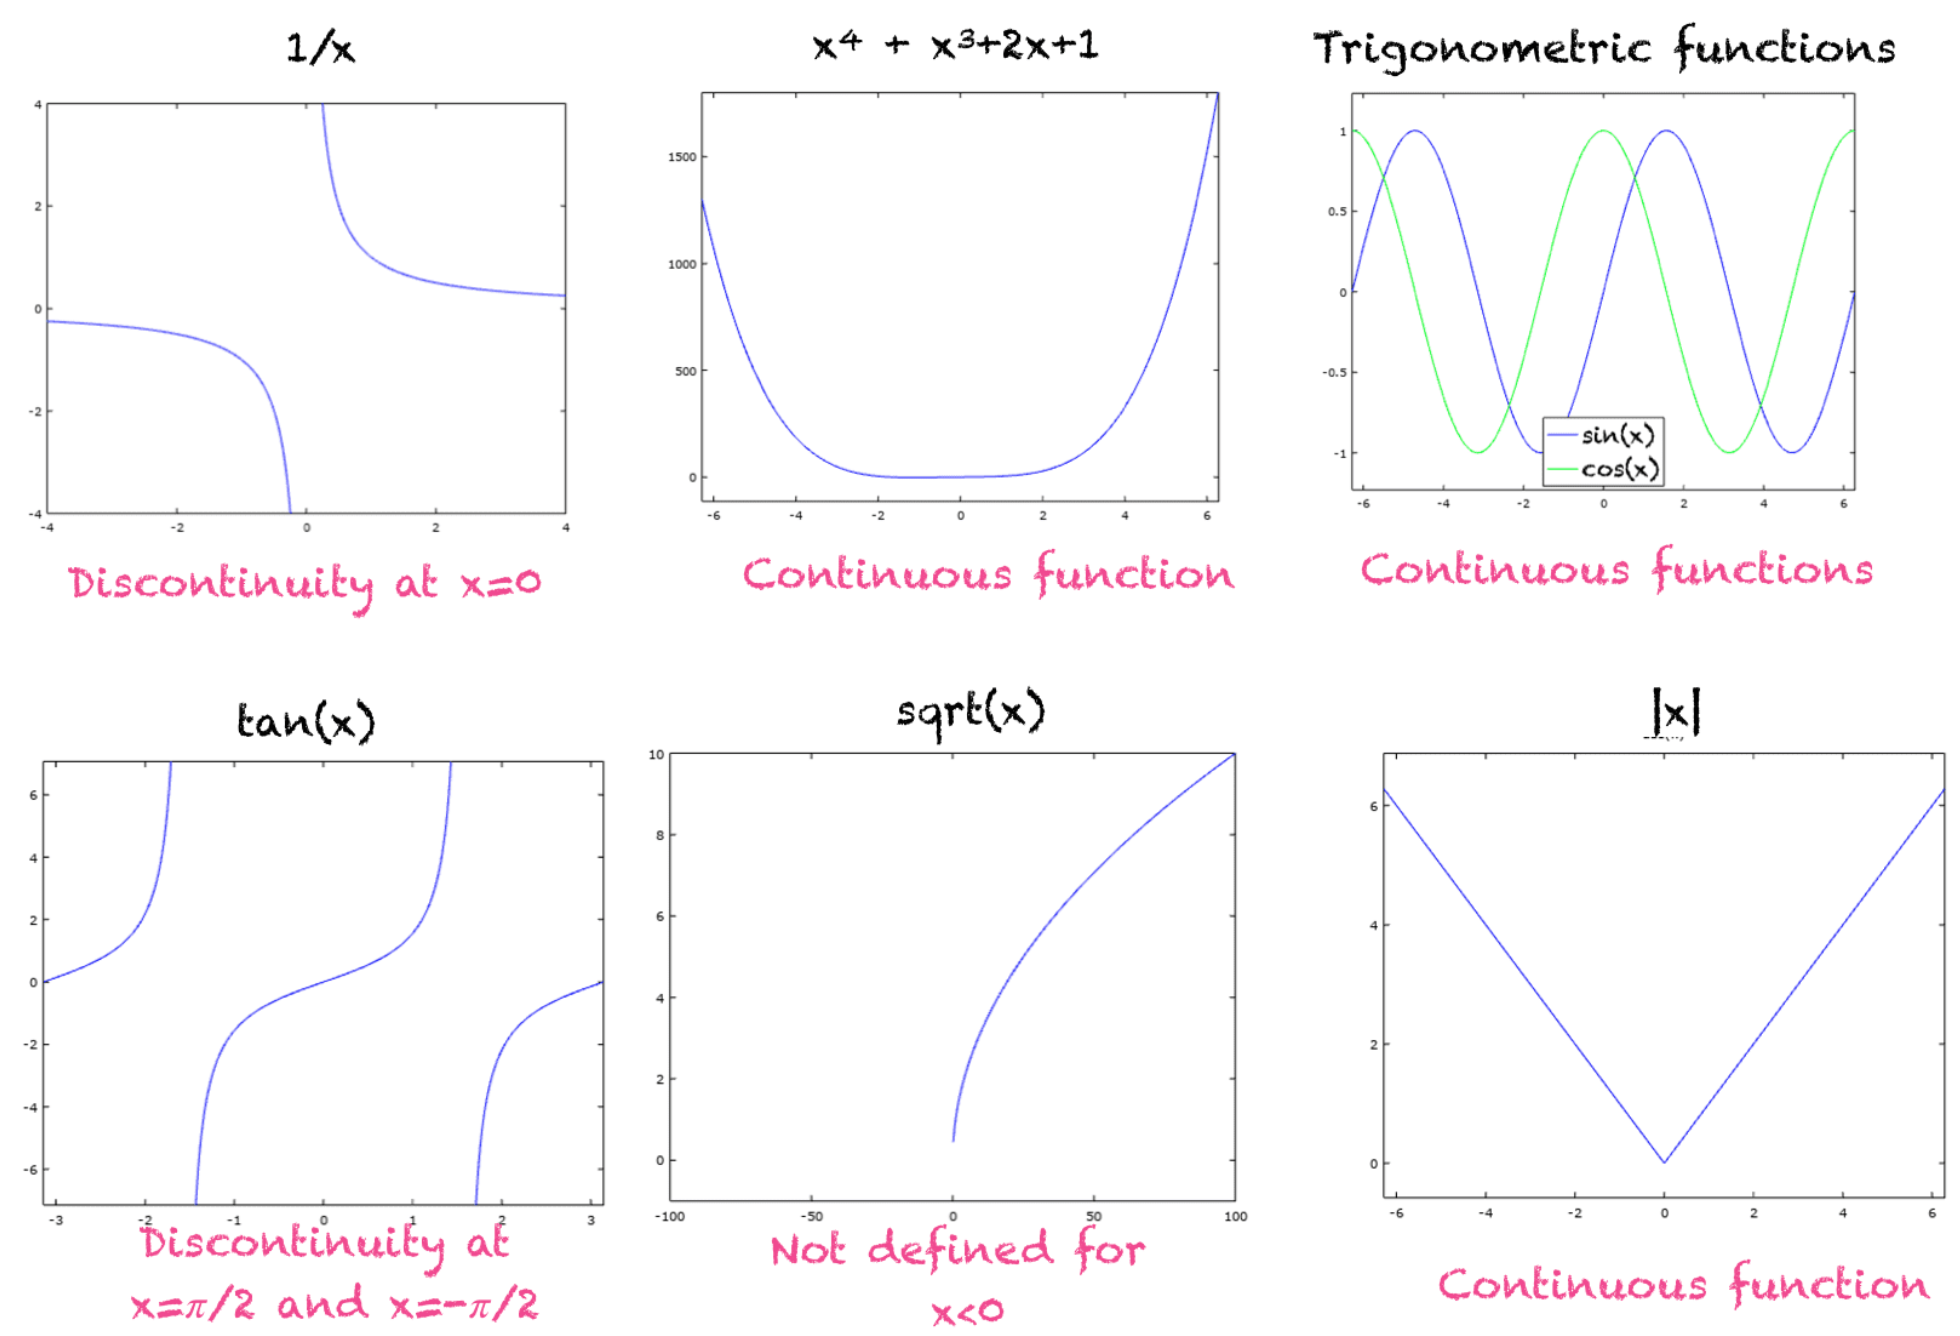
\includegraphics[scale = 0.2]{cont.png}
\end{center}
\url{https://machinelearningmastery.com/continuous-functions/}
\end{frame}

\begin{frame}
\frametitle{Useful Theorem}
\begin{Theorem}
If $f$ is continuous at $b$ and $\displaystyle\lim_{x\to a} g(x) = b$, then
$$
\lim_{x\to a} f\Big(g(x)\Big) = f\left(\lim_{x\to a} g(x)\right) = f(b).
$$
\end{Theorem}
\end{frame}

\begin{frame}[t]
\frametitle{Example}
\begin{Example}
Suppose $p > 0$. Compute $\displaystyle\lim_{x\to\infty} p^{1/x}$.
\end{Example}
\end{frame}

%\subsection{The Intermediate Value Theorem}

%\begin{frame}
%\frametitle{The Intermediate Value Theorem}
%\begin{Theorem}[Intermediate Value Theorem]
%Suppose $f$ is continuous on the closed interval $[a, b]$ and let $y$ be any number strictly between $f(a)$ and $f(b)$. Then there exists a number $c$ in $(a, b)$ such that $f(c) = y$.
%\end{Theorem}
%\end{frame}

%\begin{frame}[t]
%\frametitle{The Intermediate Value Theorem Cont.}
%\begin{Example}
%Suppose $f$ is a function with domain $[0, 1]$ and range $[0, 1]$. Prove there exists $c$ in $[0, 1]$ such that $f(c) = c$.
%\end{Example}
%\end{frame}

\section{Derivatives} 
\subsection{Definition, Examples, and Formulas}
\begin{frame}
\begin{Definition}
\frametitle{Derivatives}
\begin{enumerate}
\item[(a)] The {\bf derivative of a function} $\boldsymbol f$ at a number $a$ is
$$
f\ ' (a) = \lim_{h\to 0}\frac{f(a + h) - f(a)}{h}.
$$
\item[(b)] The function $f$ is differentiable on a set $A$ if $f\ '(a)$ exists for all $a$ in $A$.
\end{enumerate}
\end{Definition} 
\end{frame}

\begin{frame}
\frametitle{Notation}
Leibniz notation is frequently used:
$$
\frac{d f}{dx} = f\ '(x)\qquad\text{and}\qquad \frac{d f}{dx}\Big|_{x = a} = f\ '(a).
$$
The respective second and third derivatives are written
$$
\frac{d^2 f}{dx^2} = f\ ''(x)\qquad\text{and}\qquad \frac{d^3 f}{dx^3} = f\ '''(x)
$$
For the $k$-th derivatives, where $k > 3$, we use the notation
$$
\frac{d^k f}{dx^k} = f\ ^{(k)}(x).
$$
\end{frame}

\begin{frame}[t]
\frametitle{Derivatives Example}
\small
\begin{Example}
If
$$
f(x) = \begin{cases} x e^{-x^2 - x^{-2}}, & x \neq 0\\ 0,	& x= 0\end{cases}
$$
compute $f\ ' (0)$.
\end{Example}
\end{frame}

\begin{frame}
\frametitle{Numerical Approximation}
It is often helpful to numerically approximate $f\ '$. This is usually done by choosing a small value of $h$. However, in the definition, $h$ can be positive or negative. So, typically, the derivative at $x$ is approximated by
$$
\frac{1}{2}\cdot \frac{f(x + h) - f(x)}{h} + \frac{1}{2}\cdot \frac{f(x - h) - f(x)}{-h} = \frac{f(x + h) - f(x - h)}{2 h},
$$
where $h > 0$.
\end{frame}

\begin{frame}
\frametitle{Python Example}
\begin{Example}
Use Python to graph $f$ and $f\ '$ on the interval $[-2, 2]$, where
$$
f(x) = \begin{cases} x e^{-x^2 - x^{-2}}, & x \neq 0\\ 0,	& x= 0\end{cases}
$$
Use a numerical approximation $f\ '$ with $h = 0.001$.
\end{Example}
\end{frame}

\begin{frame}[fragile]
\frametitle{Python Example Cont.}
{
\linespread{0.8}
\tiny
\begin{verbatim*}
# Import modules 
import numpy as np
import matplotlib.pyplot as plt

# Use latex
plt.rcParams['text.usetex'] = True

# Use Seaborn style
plt.style.use('seaborn')

# Define f
f = lambda x: x * np.exp(-x**2 - x**-2) if x != 0 else 0

# Define h
h = 0.001

# Use numerical approx
f_prime = lambda x: (f(x + h) - f(x - h))/(2 * h)

# Get the x-values
x_vals = np.linspace(-2, 2, 100)

# Get the two sets of y-values
y1_vals = [f(x) for x in x_vals]
y2_vals = [f_prime(x) for x in x_vals]
\end{verbatim*}
}
\end{frame}

\begin{frame}[fragile]
\frametitle{Python Example Cont.}
{
\linespread{0.8}
\tiny
\begin{verbatim*}
# Generate the plot for f
plt.plot(x_vals, y1_vals, label = r"$f$")
         
# Generate the plot for f'
plt.plot(x_vals, y2_vals, label = r"$f'$")  
         
# Label the x-axis
plt.xlabel(r'$x$')
         
# Label the y-axis
plt.ylabel(r'$y$')
         
# Give the graph a title
plt.title(r"Graph of $y = f(x)$ and $y = f'(x)$")

# Create a legend
plt.legend()
         
# Save the figure
plt.savefig(r'[location on machine]')
         
# Display the plot
plt.show()    
\end{verbatim*}
}
\end{frame}

\begin{frame}
\frametitle{Python Example Result}
\begin{center}
\includegraphics[scale = 0.4]{ex3.png}
\end{center}
\end{frame}

\begin{frame}
\frametitle{Derivatives Properties}
\begin{Theorem}
Suppose $\alpha$ and $\beta$ are constants and $f\ '$ and $g\ '$ exist. 
\begin{enumerate}
\item[(a)] $\displaystyle\frac{d}{dx}\left(\alpha f + \beta g\right) = \alpha f\ ' + \beta g\ '$.
\item[(b)] $\displaystyle\frac{d}{dx}\left(f\cdot g\right) = g\cdot f\ ' + f\cdot g\ '$
\item[(c)] $\displaystyle\frac{d}{dx}\left(\frac{f}{g}\right) = \frac{f\ '\cdot g - f\cdot g\ '}{g^2}$
\item[(d)] $\displaystyle\frac{d}{dx}\left(f\circ g\right) = \left(f\ ' \circ g\right)\cdot g\ '$
\end{enumerate}
\end{Theorem}
\end{frame}

\begin{frame}
\frametitle{Useful Derivative Formulas}
Suppose $a > 0$.
\begin{multicols}{2}
\begin{itemize}
\item $\frac{d}{dx}(x^n) = n x^{n-1}$				
\item $\frac{d}{dx}(e^x)  = e^x$
\item $\frac{d}{dx}(a^x)  = a^x \ln a$
\item $\frac{d}{dx}\left(\ln|x|\right)  = \frac{1}{x}$ given $x\neq 0$
\item $\frac{d}{dx}\left(\log_a|x|\right) = \frac{1}{x\ln a}$ given $x\neq 0$
\item $\frac{d}{dx}\left(\sin x\right) = \cos x$
\item $\frac{d}{dx}\left(\cos x\right) = -\sin x$
\item $\frac{d}{dx}\left(\tan x\right) = \sec^2 x$
\item $\frac{d}{dx}\left(\arctan x\right) = \frac{1}{1 + x^2}$
\end{itemize}
\end{multicols}
\end{frame}

\subsection{Tangent Lines}

\begin{frame}
\frametitle{Tangent Lines}
The tangent line of the graph of $y = f(x)$ at $(x_0, y_0)$ is
$$
y = y_0 + f\ '(x_0)(x - x_0).
$$
\end{frame}

\begin{frame}[t]
\frametitle{Tangent Line Example}
\begin{Example}
Approximate $\sqrt{3.9}$.
\end{Example}

\end{frame}


\subsection{Optimization}

\begin{frame}
\frametitle{Optimization}

\begin{Definition}
Let $f$ be a function defined on domain $D$.
\begin{enumerate}
\item[(a)] The {\bf global maximum} of $f$ is at $c$ if $f(c)\geq f(x)$ for all $x$ in $D$. The {\bf global minimum} of $f$ is at $c$ if $f(c) \leq f(x)$ for all $x$ in $D$. The global maximum and global minimum values of $f$ are called the {\bf global extrema} of $f$.
\item[(b)] A {\bf local maximum} of $f$ is at $c$ if there is an interval $(a, b)$, where $a < c < b$, such that $f(c) \geq f(x)$ for all $x$ in $(a, b)$. Similarly, a {\bf local minimum} of $f$ is at $c$ $f(c) \leq f(x)$ for all $x$ in $(a, b)$. The local maximum and local minimum values of $f$ are called the {\bf local extrema} of $f$.
\end{enumerate}
\end{Definition}
\end{frame}

\begin{frame}
\frametitle{Extreme Value Theorem}

\begin{Theorem}[Extreme Value Theorem]
If $f$ is continuous on a closed interval $[a, b]$, then $f$ attains a global maximum value $f(c)$ and a global minimum value $f(d)$ for some numbers $c$ and $d$ in $[a, b]$.
\end{Theorem}

\end{frame}

\begin{frame}[t]
\frametitle{Increasing and Decreasing Functions}

\begin{itemize}
\item If $f\ '(x) > 0 $, then $f$ is increasing at $x$.
\item If $f\ ' (x) < 0$, then $f$ is decreasing at $x$.
\end{itemize}

\end{frame}

\begin{frame}
\frametitle{First Derivative Test}
Suppose $c$ is a critical number (i.e. $c$ is in the domain of $f$ and $f\ '(c)$ is 0 or undefined).
\begin{itemize}
\item[(a)] If $f\ '$ changes from positive to negative at $c$, then $f$ has a local maximum at $c$.
\item[(b)] $f\ '$ changes from negative to positive at $c$, then $f$ has a local minimum at $c$.
\item[(c)] If $f\ '$ does not change sign at $c$, then $f$ has no local extremum at $c$.
\end{itemize}
\end{frame}

\begin{frame}[t]
\frametitle{Optimization Example}
\small
\begin{Example}
Find the local and global extrema of the function $f(x) = x^3(x-2)^2$. Suppose the domain of $f$ is the closed interval $[-1, 3]$.
\end{Example}
\end{frame}

\begin{frame}
\frametitle{Second Derivative Test}
\begin{enumerate}
\item[(a)] If $f\ '(c) = 0$ and $f\ ''(c) > 0$, then $f$ has a local minimum at $c$.
\item[(b)] If $f\ '(c) = 0$ and $f\ ''(c) < 0$, then $f$ has a local maximum at $c$.
\item[(c)] If $f\  ''(c) = 0$, then the test fails.
\end{enumerate}
\end{frame}

\begin{frame}[t]
\frametitle{Local Extrema Example}
\begin{Example}
Find all local extrema of $g(x) = x^4 - 4x^3$.
\end{Example}
\end{frame}

%\subsection{Mean Value Theorem}

%\begin{frame}
%\frametitle{Mean Value Theorem}
%\begin{Theorem}[Mean Value Theorem]
%If $f$ is continuous on the closed interval $(a, b)$ and differentiable on the closed interval $(a, b)$, then there is a point $c$ in $(a, b)$ such that
%$$
%f\ ' (c) = \frac{f(b) - f(a)}{b - a}.
%$$
%\end{Theorem}
%\end{frame}

%\begin{frame}[t]
%\frametitle{Mean Value Theorem Cont.}
%\begin{Example}
%Suppose we know that $f$ is continuous on the closed interval $[-7, 0]$, $f(-7) = -3$, and $-\infty < $f\ '(x) \leq 2$ for all $x$ in $(-7, 0)$. What is the largest possible value of $f(0)$?
%\end{Example}
%\end{frame}

\subsection{L'H\^{o}pital's Rule}

\begin{frame}
\frametitle{L'H\^{o}pital's Rule}

\begin{Theorem}[L'H\^{o}pital's Rule]
Suppose $f$ and $g$ are differentiable on the open interval $(a, b)$ and $g\ ' (x) \neq 0$ for all $x$ in $(a, b)$, where $a\leq a < b \leq \infty$. If
$$
\lim_{x\to a} \frac{f\ '(x)}{g\ '(x)} = L
$$
and either
$$
\lim_{x\to a} f(x) = \lim_{x\to a} g(x) = 0\qquad\text{or}\qquad \lim_{x\to a} f(x) = \lim_{x\to a} g(x) = \infty,
$$
then
$$
\lim_{x\to a} \frac{f(x)}{g(x)} = L.
$$
\end{Theorem}
\end{frame}

\begin{frame}[t]
\frametitle{L'H\^{o}pital's Rule Cont.}
\begin{Example}
Prove $\displaystyle\lim_{x\to\infty} x^{1/x} = 1$.
\end{Example}
\end{frame}


\end{document}
